\chapter{经典模型概述}
\label{chap:classic-models-overview}

同一批房屋记录，可以因想得到的东西不同而变成四类不同任务：给定面积、房龄、地段，预测成交价是回归；把房价归入“便宜、适中、昂贵”几档是分类；不预设价格标签，按地段、房型、成交水平把相似房屋聚成若干群组是聚类；把多项属性压缩成少数几个能代表主要变化的坐标是降维。本卷前四章正是按“想得到什么”依次展开回归、分类、聚类与降维；第六章的集成学习不是新的输出形式，而是把已经学会的多个预测器组合起来使用。前四章按输出结果划分，集成按构造方式划分，两种划分标准并不互斥：一个集成里的成员本身可以是回归、分类或树模型。

本章只建立这些模型共同的认识：任务决定输出，输出决定损失和评价；模型是表示关系、学习参数与评价效果的一套机制。核的一般定义、合法核的依据、核矩阵与中心化在本章建立；具体模型的目标函数、梯度与对偶推导仍在各自章节展开。多分类的组合方式、概率校准、区间预测与各项评价指标，也分别放在任务对应的章节，本章不预先替代。

\section{从任务确定模型的输出}
\label{sec:classic-tasks}

\subsection{回归与分类：利用带标签的记录预测}
给定面积、房龄和地段，成交价是一个具体数字，回归要估计这个数字；把房屋归入“便宜、适中、昂贵”的类别，分类要判断它属于哪一档。回归的输出是一个连续数值，分类的输出是有限个类别中的一个；即使都从面积、房龄出发，两者最终回答的问题不同，输出的数值含义也不同。

用来综合属性的加权和形式在两类任务中可以复用，但连接这个得分的方式不同：回归把得分本身作为数值预测，误差按预测值与真实数值的距离计算；分类把得分与类别规则连接（超过阈值归为某类，或把得分转成各类概率再比较），评价的是类别判断是否正确。这里只给出最基本的形式，回归的平方误差、分类的得分与概率如何学习，留到各自章节。

标签、学习目标与评价口径必须彼此对应。同样是预测房价，估计平均价格和满足“以给定概率不超预算”的分位数，是两个不同目标；同样是分类，只输出硬类别和输出带概率的类别判断，要求模型提供的信息也不同。这些评价指标的选择在任务章节展开，本章只先区分“输出的是什么”，不把它们与后面介绍的方法清单混为一谈。

\subsection{聚类与降维：从输入中提取结构}
\label{sec:classic-overview-unsupervised}

去掉价格或类别标签后，任务性质随之改变。聚类不再预测某个外部答案，而是依据属性自身的相似程度，把记录分成若干群组；降维则把多项属性压缩成少数几个坐标，用这些坐标概括原来的变化。聚类的输出是群组的归属，降维的输出是低维坐标，两者都没有外部标准答案可供核对。

分组依据什么、保留什么变化，由各自准则决定：聚类按距离或密度判断相似，降维按方差或重构误差选择方向。被分成的群组并不自动等于真实类别，变化最大的方向也不自动有利于分类——这些准则的含义在聚类章与降维章展开。

用同一组二维点可以看清两者的差别：问“这些点可以分成几组”，得到的是若干个簇的归属；问“把它们投影到哪一条轴上最能保留变化”，得到的是一个一维坐标。前者回答结构如何划分，后者回答信息如何压缩，评价对象完全不同。回归与分类使用人为给出的答案，聚类与降维没有外部答案，监督与无监督等学习范式的整体区分可参考\BookChapterRef{chap:machine-learning-paradigms}{卷三《基础、理论与可信性》的“范式简介”章}；本章先把这两类无监督输出与监督输出区分开，为后面两章各自的准则建立入口。

\section{常见方法}
\label{sec:classic-common-methods}

下面按“计算时利用了什么关系”比较几类常见方法：用全局加权和描述整体关系，用特征内积绕过显式展开，用查询点附近的记录提供局部答案，用输入条件把空间切成局部区域，用概率模型表达不确定性，以及把多个预测组合起来。这些工具可以叠加使用，例如核可以接在线性得分上，树可以作为集成的成员；每一小节只交代该方法的核心计算与适用边界，完整推导属于对应章节。

\subsection{特征加权：用全局关系产生预测}
\label{sec:classic-overview-linear}

最朴素的价格估计是先给一个基准价格，再让面积、房龄各自贡献一个固定的增量：面积每增加一单位，价格增加一个固定数额；房龄每增加一单位，价格减少一个固定数额。把这些贡献写成一个加权和，就是
\begin{equation}
  g(\bm x)=b+\bm w^{\top}\bm x,
  \label{eq:classic-overview-linear-score}
\end{equation}
其中$b$是基准（截距），$\bm w$是各属性的贡献系数，$\bm x$是输入属性。无论回归还是分类，都可以先写出这样一个得分，再决定它怎样变成最终输出。

这个形式有一个隐含限制：在其他属性固定时，面积对价格的贡献被假设为常数，与面积本身大小、房龄高低都无关。现实中面积的边际影响可能随面积变化，两个属性之间也可能存在交互。把平方项$x_j^2$和乘积项$x_jx_k$加入加权和，就能表达这类弯曲与交互；此时模型对原始输入是非线性的，但对要估计的系数仍然是线性的，因为系数只是以线性方式进入得分。

同一个得分可以连接不同输出：回归直接取它作为数值预测，分类用阈值把它切成类别，概率模型把它送进链接函数转成概率向量。用什么损失估计系数、系数的单位是什么，由任务决定；此外，这里的系数描述的是样本中的统计关联，不等于因果效应，不能直接解释为“改变面积就会按这个数额改变价格”。

\subsection{核方法：以特征内积代替显式展开}
\label{sec:classic-overview-kernel}

线性得分只能表达原坐标中的平面关系。核方法允许我们在一个更高维的特征空间里使用线性得分，却不必真正写出这些新坐标：两个输入映射后的特征内积，直接由一个核函数$K(\bm x,\bm z)$给出。下面先说明从特征映射到核展开的依据，再交代合法核的条件与常用核，最后说明核矩阵与训练中心；核决定表示，具体任务的学习目标仍由各章给出。

\subsubsection{从特征映射到核展开}
\label{sec:classic-overview-kernel-trick}

二分类模型在输入空间中划出一条边界：边界一侧预测正类，另一侧预测负类。原始坐标的加权和只能产生直线（二维时）或超平面（高维时）边界。若两类样本恰好能被一条直线分开，线性模型足够；但类别也可能按“到原点的距离是否小于 $1$”来区分，这时正类挤在单位圆内、负类散在圆外，任何一条直线都无法把整个圆内区域与圆外区域干净分开——无论直线画在哪里，圆的这一侧和那一侧都会同时出现两类点。

判断一个点在圆内还是圆外，需要的是半径平方 $x_1^2+x_2^2$。线性模型不认识平方项，但我们可以替它造出来：把 $x_1^2+x_2^2$ 整体当作一个新特征，再继续使用熟悉的线性得分。也就是说，不是让分类器在原坐标里硬画曲线，而是先把数据搬到一组新坐标，使在新坐标里分界重新变成直线。

图\ref{fig:classification-kernel-map}采用映射$\bm{\phi}(\bm{x})=(x_1,x_1^2+x_2^2)^{\top}$，将圆$x_1^2+x_2^2=1$对应到直线$\phi_2=1$。得分$g(\bm{x})=1-x_1^2-x_2^2$于是写成$g(\bm{x})=(0,-1)\bm{\phi}(\bm{x})+1$：对原坐标非线性，对新特征却是线性的。样本类别保持不变，改变的只是描述它们的坐标；图中边界是教学构造，并非由数据训练得到的最优分类边界。

\begin{figure}[htbp]
  \centering
  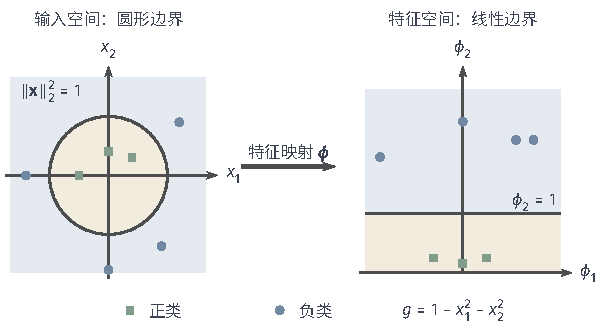
\includegraphics[width=103.166mm]{figures/04-classic-models/00-shared/tikz/classification-kernel-map/figure.pdf}
  \caption{非线性边界在特征映射前后的对应，两个面板的坐标均无量纲。正类方点为$(-0.5,0)$、$(0,0.4)$、$(0.4,0.3)$，负类圆点为$(-1.4,0)$、$(0,-1.6)$、$(1.2,0.9)$、$(0.9,-1.2)$。右图逐点使用$\phi_1=x_1$、$\phi_2=x_1^2+x_2^2$；水平线$\phi_2=1$对应左图半径为1的圆。数据与边界均为教学构造。}
  \label{fig:classification-kernel-map}
\end{figure}

圆形例子只需计算一个新特征，成本可以忽略。但若为了描述更复杂的弯曲关系而加入大量平方项、两两交互项甚至更高次项，显式列出所有新坐标就可能非常昂贵：仅二次映射，$d$ 个原变量就要产生约 $d^2/2$ 个新坐标，次数再升高数量还会快速增长；计算、存储和后续求解都要承担这份开销。于是出现一个关键问题：能不能在不真正写出、也不保存这些新坐标的情况下，照样完成计算？

\emph{从“只需内积”到核展开。}要回答这个问题，先检查线性算法到底怎样使用特征。给定$n$个训练输入$\bm x_1,\ldots,\bm x_n$，设$\bm\phi$将输入映射到带内积的特征空间$\mathcal H$，在那里使用线性得分$\langle\bm w,\bm\phi(\bm x)\rangle+b$。

在一类常见的训练问题里，训练损失只依赖各训练点的得分，而惩罚是参数范数的非减函数。把$\mathcal H$中的任意参数向量分解为“训练特征张成空间内的部分”与“正交于该空间的部分”：正交部分与每个训练特征的内积都是零，把它加到 $\bm w$ 上不会改变任何训练点的得分，却只会增大参数范数，从而增大惩罚。删去这一正交部分，训练得分不变、惩罚不增，因此若最优解存在，总能在这 $n$ 个训练特征张成的空间里找到它（张成空间＝这些特征向量线性组合能够到达的全部方向），即存在一组系数 $a_i$ 使
\begin{equation}
  \bm w=\sum_{i=1}^n a_i\bm\phi(\bm x_i).
  \label{eq:classic-overview-weight-expansion}
\end{equation}
这一展开只说明“有解时解可取在训练特征张成内”，并不单独证明解存在或唯一；存在性与唯一性仍由具体学习目标决定。

把这一展开代回线性得分，内积的线性性质允许把求和提到内积外面：
\begin{equation}
  \begin{aligned}
    K(\bm x,\bm z)
      &=\langle\bm\phi(\bm x),\bm\phi(\bm z)\rangle_{\mathcal H},\\
    f(\bm x)&=\sum_{i=1}^n a_iK(\bm x_i,\bm x)+b.
  \end{aligned}
  \label{eq:classic-overview-kernel}
\end{equation}
这里三者职责不同：核 $K$ 只给出两个输入映射后的特征内积，样本系数 $a_i$ 由具体学习目标确定，截距 $b$ 处理特征均值未被零化的整体偏移。预测时只需逐个计算新输入与训练输入的核值，既不必写出映射后的坐标，也不必保存高维的 $\bm w$。这种用核值完成特征内积计算的办法称为\term{核技巧}（kernel trick）；当$K$对原输入非线性时，特征空间中的线性得分也能描述原空间中的非线性关系，而显式特征展开这一步被完全绕过。

注意，式~\eqref{eq:classic-overview-kernel}只保证“预测”能改写为核值计算；要连训练也一起省去显式特征，训练问题本身也必须只通过核值使用特征。例如训练损失只使用各训练点的得分，并以正系数惩罚参数范数平方时，前面关于正交部分的论证正好适用：正交部分不改变训练得分却增加惩罚，最优解自然落在训练特征张成的空间内，于是整个训练都可用上述有限展开完成。具体到支持向量机，这一对偶形式将在分类章推导。核决定的是特征表示，分类、回归等任务仍由各自的损失和约束确定学习目标。

\subsubsection{合法核、常用核与超参数}
\label{sec:classic-overview-kernel-validity}
\label{sec:classic-overview-common-kernels}

\emph{什么样的函数才能充当核。}从“衡量相似性”的直觉随手设计一个 $K$ 并不困难，但不是每个看起来合理的相似性公式都能作为内积的替代。先注意这里说的“核”是特征内积的代称，与回归章局部加权里“按距离给记录加权重”的核只是同名：那个距离权重核只决定邻域内的加权平均，并不对应某个特征空间。原因在于，$K$ 必须真的等于某个特征空间中的内积，而内积有不能违反的代数性质。

内积首先是对称的：$\langle\bm u,\bm v\rangle=\langle\bm v,\bm u\rangle$。更重要的是，任意特征向量线性组合的长度平方都不可能为负。因此，对任意有限个输入$\bm x_1,\ldots,\bm x_m$和任意实系数$c_1,\ldots,c_m$，必须有
\[
  \begin{aligned}
    \sum_{i,j=1}^m c_ic_jK(\bm x_i,\bm x_j)
      &=\left\lVert\sum_{i=1}^m c_i\bm\phi(\bm x_i)\right\rVert^2\\
      &\geq0.
  \end{aligned}
\]
将这些输入的核值排成矩阵，称为这组输入的\term{Gram矩阵}（Gram matrix），也就是两两特征内积组成的矩阵；上述条件等价于矩阵对称且半正定，即用任意实向量 $\bm c$ 左乘右乘都不会得到负数。

反过来，若一个对称函数在整个预期输入域上对每一组有限输入都满足“Gram矩阵半正定”，就可以从形式特征的有限线性组合出发构造半内积（允许某个非零向量范数为零的退化内积），再把零范数的等价类消去、对空间完备化（补上所有极限点，使空间闭合），得到一个以该核为内积的特征空间。这里只交代存在性依据；连续性等Mercer定理的附加条件是针对特定定义域与连续核的进一步要求，不能误列为所有合法核的必要条件。本书将这样的函数称为正定核（positive definite kernel），允许有限核矩阵奇异（即存在非零 $\bm c$ 使二次型为零），不额外要求矩阵可逆。

合法性检查的是“所有实系数形成的二次型是否非负”，要避免几种常见误解。它不是检查每个核值本身是否非负——合法核在不相似的两点上完全可以取负值（例如未加常数的线性核）。它也不是凭“看起来像相似性”就能成立。只检查某一份训练集上的矩阵，只能确认这一组输入合法；新输入还必须落在核已确认合法的定义域内。此外，合法核只提供“它确实对应某个特征内积”的依据，并不保证这个特征表示适合当前任务，也不保证对应的学习目标容易求解——合法性与有效性是两件事。

对$\bm x,\bm z\in\mathbb R^d$，选择不同的核，等于暗中选择了不同的特征空间和特征关系。表\ref{tab:classic-overview-common-kernels}列出常见形式及条件；核尺度记为$\beta$，多项式次数记为$p$，与输入维数$d$区分。

\begin{table}[htbp]
  \centering
  \small
  \begin{tabularx}{\linewidth}{@{}>{\RaggedRight\arraybackslash}p{18mm}>{\RaggedRight\arraybackslash}X>{\RaggedRight\arraybackslash}p{27mm}@{}}
    \toprule
    名称 & $K(\bm{x},\bm{z})$ & 参数与正定性\\
    \midrule
    线性核 & $\bm{x}^{\top}\bm{z}$ & 半正定\\
    多项式核 & $(\beta\bm{x}^{\top}\bm{z}+r)^p$ & $\beta,r\ge0$，正整数$p$\\
    高斯RBF核 & $\exp(-\beta\lVert\bm{x}-\bm{z}\rVert_2^2)$ & $\beta>0$，半正定\\
    Laplacian核 & $\exp(-\beta\lVert\bm{x}-\bm{z}\rVert_1)$ & $\beta>0$，半正定\\
    Sigmoid形式 & $\tanh(\beta\bm{x}^{\top}\bm{z}+r)$ & 一般不保证半正定\\
    \bottomrule
  \end{tabularx}
  \caption{常用核函数与合法性条件。这里的“半正定”要求任意有限输入的Gram矩阵半正定；Sigmoid一行列出的是常见相似性形式，使用前仍需针对定义域与参数核验。}
  \label{tab:classic-overview-common-kernels}
\end{table}

\term{线性核}（linear kernel）就是原始特征的内积，不增加任何新特征，对应普通的线性模型，常作为比较基准。\term{多项式核}（polynomial kernel）隐式加入了有限阶的特征交互：把 $(\beta\bm x^\top\bm z+r)^p$ 展开后，各项对应原变量的各次乘积，因此 $p=2$ 时能表达平方项和两两乘积，$p$ 更大时表达更高次的组合。在$\beta>0$时，$r=0$只保留$p$次项，$r>0$则包含从常数项到$p$次项的各阶特征；参数取零时，相应特征块可以消失。核计算省去的是这些坐标的显式展开，完整训练成本仍取决于样本数和学习目标。

\term{高斯径向基核}（Gaussian radial basis function kernel，Gaussian RBF kernel）不看方向上的投影，而按两点的欧氏距离衡量局部接近程度：两点重合时核值为 $1$，距离越远核值平滑衰减到 $0$。常将$\beta$写成$1/(2\sigma^2)$，其中$\sigma>0$是距离尺度：$\sigma$ 越大（$\beta$ 越小），核值衰减越慢，一个点能影响的范围越宽；$\sigma$ 越小（$\beta$ 越大），作用范围越局部。它对应的特征空间是无限维的，因而能表达相当灵活的非线性关系，但作用范围是否合适仍需结合数据判断，不能仅凭“能拟合弯曲边界”就断定新样本误差更小。

\term{Laplacian核}（Laplacian kernel）形式相近，只是把欧氏距离换成$L^1$距离，即各坐标绝对差之和；$L^1$距离沿坐标轴方向变化，改变了衡量“接近”的几何，对某些坐标轴对齐的结构更敏感。

常称为\term{Sigmoid核}（sigmoid kernel）的形式把内积送入双曲正切函数，在神经网络兴起后常被使用，但它一般不保证正定核所需的半正定性；只取正参数也不足以替代对定义域和参数取值的合法性核验，使用前必须单独检查或改用其他核。核尺度、多项式次数、正则化强度等在一次拟合前固定的配置，可以用验证数据在训练内选择；配置确定后，还要用未参与选择的新数据评价预测误差，不能把选择配置时用过的数据再当作最终评价依据。

\subsubsection{核矩阵与训练中心}
\label{sec:classic-overview-kernel-matrix}

把预测公式用于全部训练点，可以看出核方法的规模压力落在哪里。训练时，将$n$个输入两两之间的核值排成训练Gram矩阵$\bm K\in\mathbb R^{n\times n}$，其中$\bm K_{i,j}=K(\bm x_i,\bm x_j)$。令$\bm a=(a_1,\ldots,a_n)^{\top}$、$\bm1\in\mathbb R^n$为全一向量，式\eqref{eq:classic-overview-kernel}在训练点上的预测便是$\bm K\bm a+b\bm1$。完整存储这个矩阵需要$O(n^2)$空间，构造它需要$O(n^2)$次核计算；也就是说，核技巧把“显式展开可能极高维的特征”的压力，转换成了“成对计算并存储样本关系”的压力，后续求解线性或二次问题的成本还要另外计算。当样本量很大时，这一 $n^2$ 规模往往比特征维数更先成为瓶颈，省去显式坐标并不等于没有计算代价。

有些学习目标要求比较样本围绕共同中心的变化，而不是它们相对原点的绝对位置。例如核PCA要在特征空间中找“数据散布最大的方向”，这一分析应当围绕特征均值进行；原点位置改变不应影响结论。这时需要在特征空间中减去训练均值。训练特征均值与各点的偏离量为
\[
  \bar{\bm\phi}=\frac1n\sum_{i=1}^n\bm\phi(\bm x_i),
  \qquad
  \widetilde{\bm\phi}_i=\bm\phi(\bm x_i)-\bar{\bm\phi}.
\]
中心化后的内积仍可只用核值计算。令$\bm I_n$为单位矩阵，中心化矩阵和中心化核矩阵为
\begin{equation}
  \bm H=\bm I_n-\frac1n\bm1\bm1^{\top},
  \qquad \bm K_{\mathrm c}=\bm H\bm K\bm H.
  \label{eq:classic-overview-kernel-centering}
\end{equation}
矩阵 $\bm H$ 的作用就是“减去平均值”：左乘或右乘 $\bm H$ 相当于减去行均值或列均值。有限维特征按行排成矩阵$\bm\Phi$时，减去每列训练均值得到$\bm H\bm\Phi$，其Gram矩阵就是$\bm H\bm\Phi\bm\Phi^{\top}\bm H=\bm H\bm K\bm H$。即使特征空间是无限维的，无法写出矩阵 $\bm\Phi$，直接展开中心化特征的内积也得到同一个公式 $\bm H\bm K\bm H$，这正是核技巧的价值所在。还要注意，非线性映射与减均值一般不能交换次序，因此只在原输入空间做中心化，并不能代替在特征空间中的这一步。

新输入$\bm x$在预测时也必须减去同一个训练特征均值，保持训练和预测使用共同参照；不能为每个新查询重新定义中心，否则训练得到的坐标与预测坐标不在同一参照系中。它与第$i$个训练输入的中心化核值为
\[
  \begin{aligned}
    K_{\mathrm c}(\bm x_i,\bm x)
      ={}&K(\bm x_i,\bm x)
       -\frac1n\sum_{j=1}^n K(\bm x_i,\bm x_j)\\
       &-\frac1n\sum_{j=1}^n K(\bm x_j,\bm x)
       +\frac1{n^2}\sum_{j,l=1}^n K(\bm x_j,\bm x_l).
  \end{aligned}
\]
四项可以逐项对照 $\langle\bm\phi(\bm x_i)-\bar{\bm\phi},\bm\phi(\bm x)-\bar{\bm\phi}\rangle$ 的展开来理解：第一项是原内积，第二、三项分别扣除两个端点与训练均值的内积，最后一项把均值自身的内积加回来，因为它在前两步里被减了两次。所有求和都固定使用训练输入，新点不参与均值的计算。是否中心化由学习目标决定：核PCA这类分析围绕特征均值变化的方法需要中心化，而直接做分类、回归的核方法未必需要；采用核并不意味着所有方法都执行同一套中心化流程。


\subsection{邻域方法：参考查询附近的记录}
\label{sec:classic-overview-neighborhood}

与“用一个全局加权和概括所有样本”相反，邻域方法只看查询点附近的少量记录。要估计一套从未见过的房屋价格，找出与它面积、房龄最接近的若干套已成交房屋，用它们的成交价作平均；要判断一封新邮件是否垃圾邮件，找出词频分布最接近的若干封已标注邮件，按多数类别投票。这里不假设一条统一的关系曲线贯穿全部样本，只相信邻近的记录提供局部答案。

邻域方法需要决定三件事：保留哪些训练记录、用什么距离衡量接近、怎样组织记录以便快速找到邻居。距离可以是各属性差的平方和开方，也可以是按重要性加权后的距离；“近”的定义不同，选出的邻居就不同。聚类、图表示与半监督学习都可以复用这种邻近关系，但它们还需要各自的输出规则：聚类把邻近关系组织成群组，半监督把邻近关系传播到未标注点，不能把“找邻居”本身当成最终任务。

\subsection{树与规则：按输入条件选择局部预测}
\label{sec:classic-overview-trees-rules}

树方法把输入空间按一系列条件切成小块：先问面积是否超过某个值，再在每一块里问房龄或地段，逐层细分，直到每个叶块里的样本足够同质。预测时沿条件一路走到某个叶块，输出该块内的代表值（回归取均值，分类取多数类）。规则方法是同一思想的平铺形式：用“若面积大且地段好，则价格高”这样的条件组合直接给出判断。

与全局加权和相比，树不需要把整个空间套进一条直线或一个曲面，弯曲关系由一系列分段直线拼接出来；与邻域方法相比，树的划分边界由数据按准则选出，而不是预先固定一个邻域半径。它的代价是叶块之间可能出现阶梯状跳变，且每个叶块内的样本量决定了代表值是否稳定。

\subsection{概率模型：区分响应波动与参数不确定性}
\label{sec:classic-overview-probability}

前面几类方法直接给出一个预测值；概率模型还进一步描述这个值的波动。对一套给定的房屋，成交价本身在不同交易中会有起伏，概率模型为每个输入写出响应的分布，而不只是一个点估计；例如把条件分布写成$p(y\mid\bm x;\bm\theta)$，$\bm\theta$是分布参数。

参数的不确定性用先验与后验表达：先验$\pi(\bm\theta)$描述估计前对参数的认识，似然$p(\text{数据}\mid\bm\theta)$描述数据怎样由参数产生，贝叶斯定理把两者结合成后验$p(\bm\theta\mid\text{数据})$。这里要区分两种不确定：响应波动是给定参数后$y$自身的随机，参数不确定性是$\bm\theta$尚未被数据唯一确定；判别模型直接建模$p(y\mid\bm x)$，生成模型先建模$p(\bm x,y)$再推出条件分布，两者对不确定性的处理位置不同。概率模型还可以引入未被观测的潜成分（混合分量、隐变量），连续隐变量与降维的坐标表示相互衔接。

\subsection{集成方法：组合多个预测}
\label{sec:classic-overview-ensemble}

单个模型的预测可能因训练波动或遗漏结构而不稳定，集成方法训练多个成员，再把它们的输出组合成一个结果。按成员怎样产生、怎样组合，本书区分三条路线：让成员在略有不同的数据上独立训练再平均（Bagging、随机森林）；让成员逐个产生，每一个专门修正前面组合的错误（Boosting）；让数据自己学会怎样组合已有成员的预测（Stacking）。三条路线的共同问题是成员之间的相关性、组合规则带来的偏差与部署成本，完整机制在第\ref{chap:ensemble-learning}章展开。

\section{研究历史}
\label{sec:classic-history}

本节按五个阶段梳理经典模型的发展脉络，目的是定位思想、避免错置归属：同一时期的工作面对的问题不同，不同阶段的方法也并非按一条直线替代。历史不重讲各模型的正式推导，那些推导属于各自章节。

\subsection{统计估计与多元分析的形成（19世纪初—1940年代）}
\label{sec:classic-history-estimation}

最小二乘法在19世纪初同时由勒让德与高斯发展出来：把多次观测的误差平方相加，取使总和最小的参数作为估计；观测由此通过同一个共同准则汇总，而不是各自为政\scite{legendre1805,gauss1809}。图\ref{fig:classic-history-observations}给出这一思想的场景：一组观测围绕待估数值散布，最小二乘选择让各误差平方和最小的位置。这里只说明平方准则在历史上怎样被用来取舍观测；它为什么恰好导向均值、在什么概率假设下等价于最大似然估计，留到第\ref{chap:regression}章推导。

\begin{figure}[htbp]
  \centering
  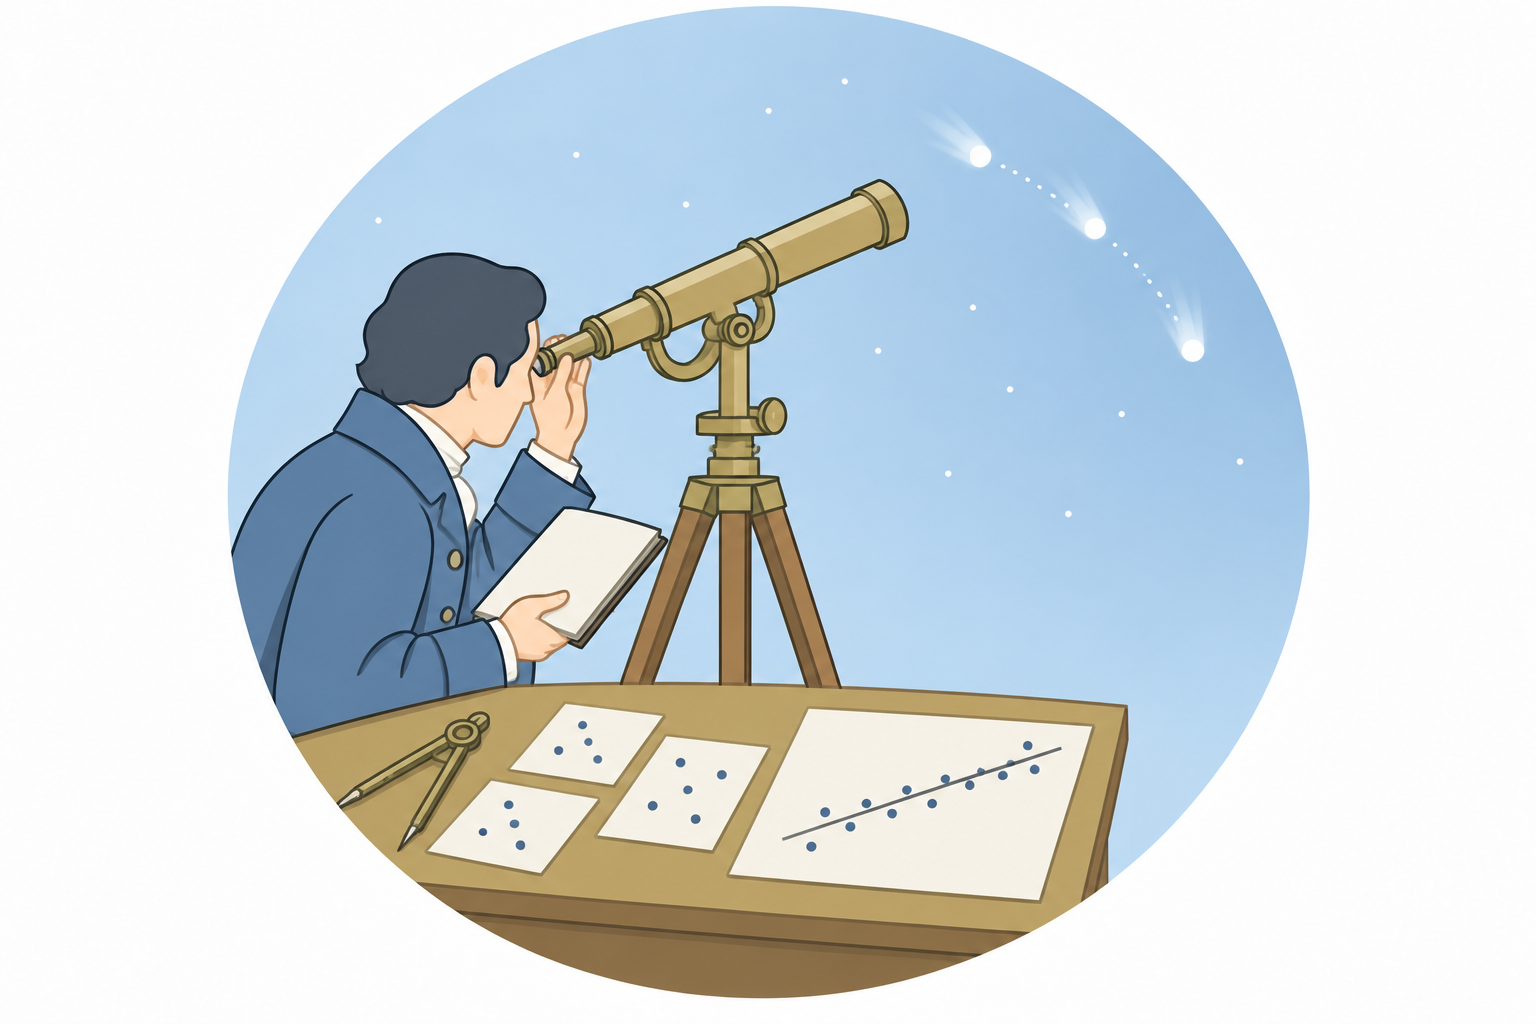
\includegraphics[width=94mm]{figures/04-classic-models/00-shared/generated/least-squares-observations/figure.png}
  \caption{围绕待估数值的多次观测（教学构造）：竖线为观测位置，黑色圆点为最小二乘估计位置；残差为观测到估计位置的水平差。}
  \label{fig:classic-history-observations}
\end{figure}

19世纪末高尔顿在亲子身高数据中观察到“向均值回归”的现象，催生了回归这一概念\scite{galton1886}。进入20世纪，皮尔逊1901年从几何拟合角度提出主成分分析，霍特林1933年把它发展为保留输入自身方差的正交坐标\scite{pearson1901pca,hotelling1933pca}；费舍尔1936年的判别分析与拉奥1948年的推广，则面向“怎样把不同类别分开”的目标\scite{fisher1936,rao1948}。图\ref{fig:classic-history-iris}展示的鸢尾花测量数据，正是费舍尔工作使用的经典多元样本。

\begin{figure}[htbp]
  \centering
  
\includegraphics[width=94mm]{figures/04-classic-models/00-shared/generated/iris-measurements/figure.png}
  \caption{三种鸢尾花的花瓣长度与花瓣宽度测量（教学示意，坐标轴无量纲）：不同类别在平面上有部分重叠，可分方向与方差较大的方向并不完全一致。}
  \label{fig:classic-history-iris}
\end{figure}

这一阶段形成了两条并行的研究目标：一条从观测误差出发估计共同参数（回归），另一条处理多变量的结构——要么保留输入自身的变化（主成分），要么区分给定类别（判别）。两者使用相似的几何工具，但优化目标不同，这一区分贯穿后续各章。

\subsection{模式识别与样本学习（1950—1960年代）}
\label{sec:classic-history-pattern}

1958年罗森布拉特提出感知机，用样本反馈直接调整线性分类的系数，标志着从“预设统计分布”转向“从样本中学习判别规则”\scite{rosenblatt1958}；几乎同时，基于邻近样本投票的早期近邻分类思路出现，而Cover与Hart在1967年给出的是近邻规则的错误率分析，并非近邻思想的首次提出，引用时不应把二者混为一谈\scite{coverhart1967}。1967年MacQueen提出以中心为代表的K-means聚类，它与监督判别使用的信息不同：没有类别标签，只按到中心的距离分组\scite{clust-macqueen1967}。

同一时期，Aizerman等人1964年的势函数方法已经把非线性特征与按样本展开的系数结合起来，是后来核表示的早期线索；但它与1990年代以间隔为准则的支持向量机属于不同问题，不能把核思想的形成全部归到1990年代\scite{aizerman1964potential}。这一阶段的共同特征是：模型直接面对样本，学习规则由样本驱动，而不是先假定完整的分布形式。

\subsection{灵活建模与计算统计（1970—1980年代）}
\label{sec:classic-history-flexible}

1972年Nelder与Wedderburn的广义线性模型把响应分布、链接函数与线性预测项统一起来，使回归不必局限于正态响应与恒等链接\scite{nelder1972glm}；Cleveland1979年的稳健局部加权回归用邻近样本的局部拟合替代一条全局直线\scite{cleveland1979lowess}；Hastie与Tibshirani1986年的广义加性模型则把单个变量的平滑效应逐项相加，放松了全局线性的约束\scite{hastie1986gam}。三者分别从响应分布、局部拟合和变量平滑三个方向扩展了全局线性模型，相应的公式在回归章展开。

1977年Dempster、Laird与Rubin系统给出EM算法的命名与迭代估计框架，为混合模型与含潜变量的估计提供了统一思路；但EM不是这一时期唯一的迭代估计算法，只应把它放在“系统化”的位置上\scite{clust-dempster1977}。1984年Breiman等人的CART专著系统整理了树的生长与剪枝，使按输入条件分区的模型有了可操作的估计流程\scite{breiman1984cart}。与分布模型、平滑模型并行，计算搜索让灵活结构成为可能，是这一阶段的共同背景。

\subsection{统计学习、非线性表示与集成（1990年代）}
\label{sec:classic-history-statistical}

1991年Friedman的MARS用自适应分段基函数表达非线性交互\scite{friedman1991mars}；1995年Cortes与Vapnik的支持向量网络以最大间隔为准则，把早期核表示与分类目标结合起来\scite{cortes1995}。这一阶段的关键词是自适应表示、间隔准则与容错训练；但核的非线性特征早在势函数时期已经出现，不能把相关思想都记在1990年代。聚类一侧，1996年Ester等人的DBSCAN提出按密度分组，与以中心划分、以混合模型拟合的路线在历史上形成对照\scite{ester1996}。

集成的三条路线也在这一阶段成型：Wolpert1992年提出Stacking，让数据学习成员怎样组合\scite{wolpert1992stacked}；Breiman1996年的Bagging通过随机扰动样本再聚合\scite{breiman1996bagging}；AdaBoost在1990年代初被提出，Freund与Schapire1997年的论文给出系统表述\scite{freund1997boosting}。三者分别对应学习组合、随机扰动聚合与顺序修正，第六章分别展开。

\subsection{非线性表示与规模化学习（2000年代以来）}
\label{sec:classic-history-scaling}

2000年的Isomap与局部线性嵌入（LLE）把全局线性的坐标表示推广到非线性流形：Isomap利用测地距离，LLE利用局部邻域关系重构坐标，具体准则在降维章推导\scite{dimTenenbaum2000,dimRoweis2000}。集成一侧，2001年Breiman的随机森林在自助采样之外加入节点级特征随机化，同年Friedman的梯度提升以负梯度方向逐轮拟合\scite{breiman2001randomforests,friedman2001gradientboost}；随后2016年的XGBoost、2017年的LightGBM把样本规模与训练成本作为明确的学习问题处理\scite{chen2016xgboost,ke2017lightgbm}。各自贡献分别对应成员随机化、顺序修正与计算组织，不合并为一个笼统的“提升方法”。

图\ref{fig:classic-models-history}按阶段汇总本节选取的代表工作。阅读这张图时按阶段定位即可，不要把不同年代的工作排成一条线性优劣序列；图中区分了思想提出、论文发表、系统化表述与理论分析各自可能相隔的时间。

\begin{figure*}[htbp]
  \centering
  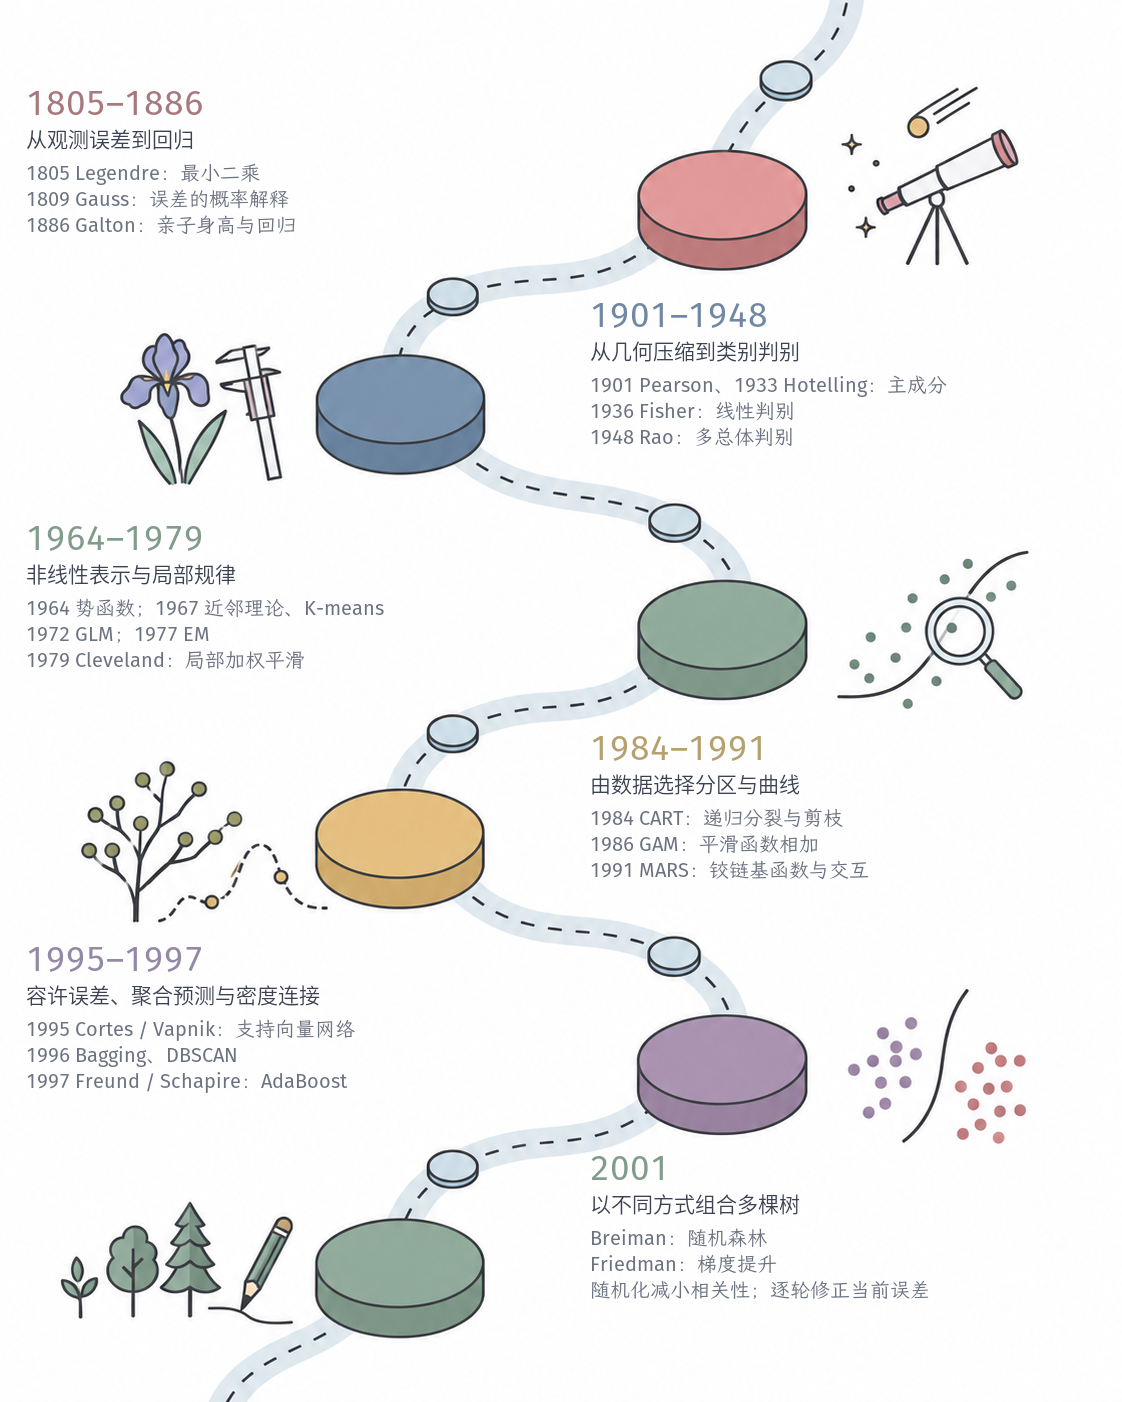
\includegraphics[width=157.406mm,height=.88\textheight,keepaspectratio]{figures/04-classic-models/00-shared/generated/classic-models-history/figure.png}
  \caption{经典模型代表工作的阶段分布（示意）。同一项工作的思想提出、发表、系统化与理论分析可能落在不同年份；图中只选取本节涉及的代表，不代表完整编年，也不按年代排序优劣。}
  \label{fig:classic-models-history}
\end{figure*}

\FloatBarrier
\section{本章小结}
\label{sec:classic-overview-summary}

任务决定模型的输出：回归给数值、分类给类别、聚类给群组、降维给坐标；输出不同，损失与评价对象随之不同，不能把估计均值、预测类别、分组与压缩坐标混为一个“拟合好坏”。本章按计算关系比较了特征加权、核方法、邻域、树与规则、概率模型与集成六类常见方法，每一类只交代核心计算与边界，表示如何学习、目标如何优化留待各章。

核的一般定义、合法核的半正定依据、有限展开的成立条件、核矩阵规模与训练中心化已在本章建立；核只决定特征表示，具体学习目标由任务章节给出。历史部分按五个阶段定位了估计与多元分析、模式识别与样本学习、灵活建模与计算统计、统计学习与集成、非线性表示与规模化学习中的代表工作，避免把不同问题、不同年代的思想错置归属。

后续章节按输出展开：回归章从数值响应落实“表示关系—学习参数—评价效果”的完整流程，此后依次进入分类、聚类、降维与集成学习。

\paragraph{扩展阅读}
一般统计学习教材可作为概念对照\scite{hastie2009,bishop2006}；历史归属以原始论文发表信息为准，本章不新增文献条目。
